\section{UX diagrams}
This diagram follows the requirements in RASD. 
The user has to be logged to use myTaxiService. 
The services common for all the users, like profile management, and passenger's ones, like taxi call, are accessible both via web or mobile app; however taxi driver's services are accessible only via mobile phone, in fact the taxi driver has to use the service while working in the taxi.
This is why the UX is divided in two parts 
\begin{itemize}
\item the {\bf white} one: represents the model common for web and mobile application
\item the {\bf colored} one: enlightens the part of the diagram only for mobile application; in case of web application the TaxiDriver Home has not more operations than the User Home.
\end{itemize}
\autoref{fig:ux-diagram} shows the UX diagram for the application.

\begin{figure}[h]
\centering
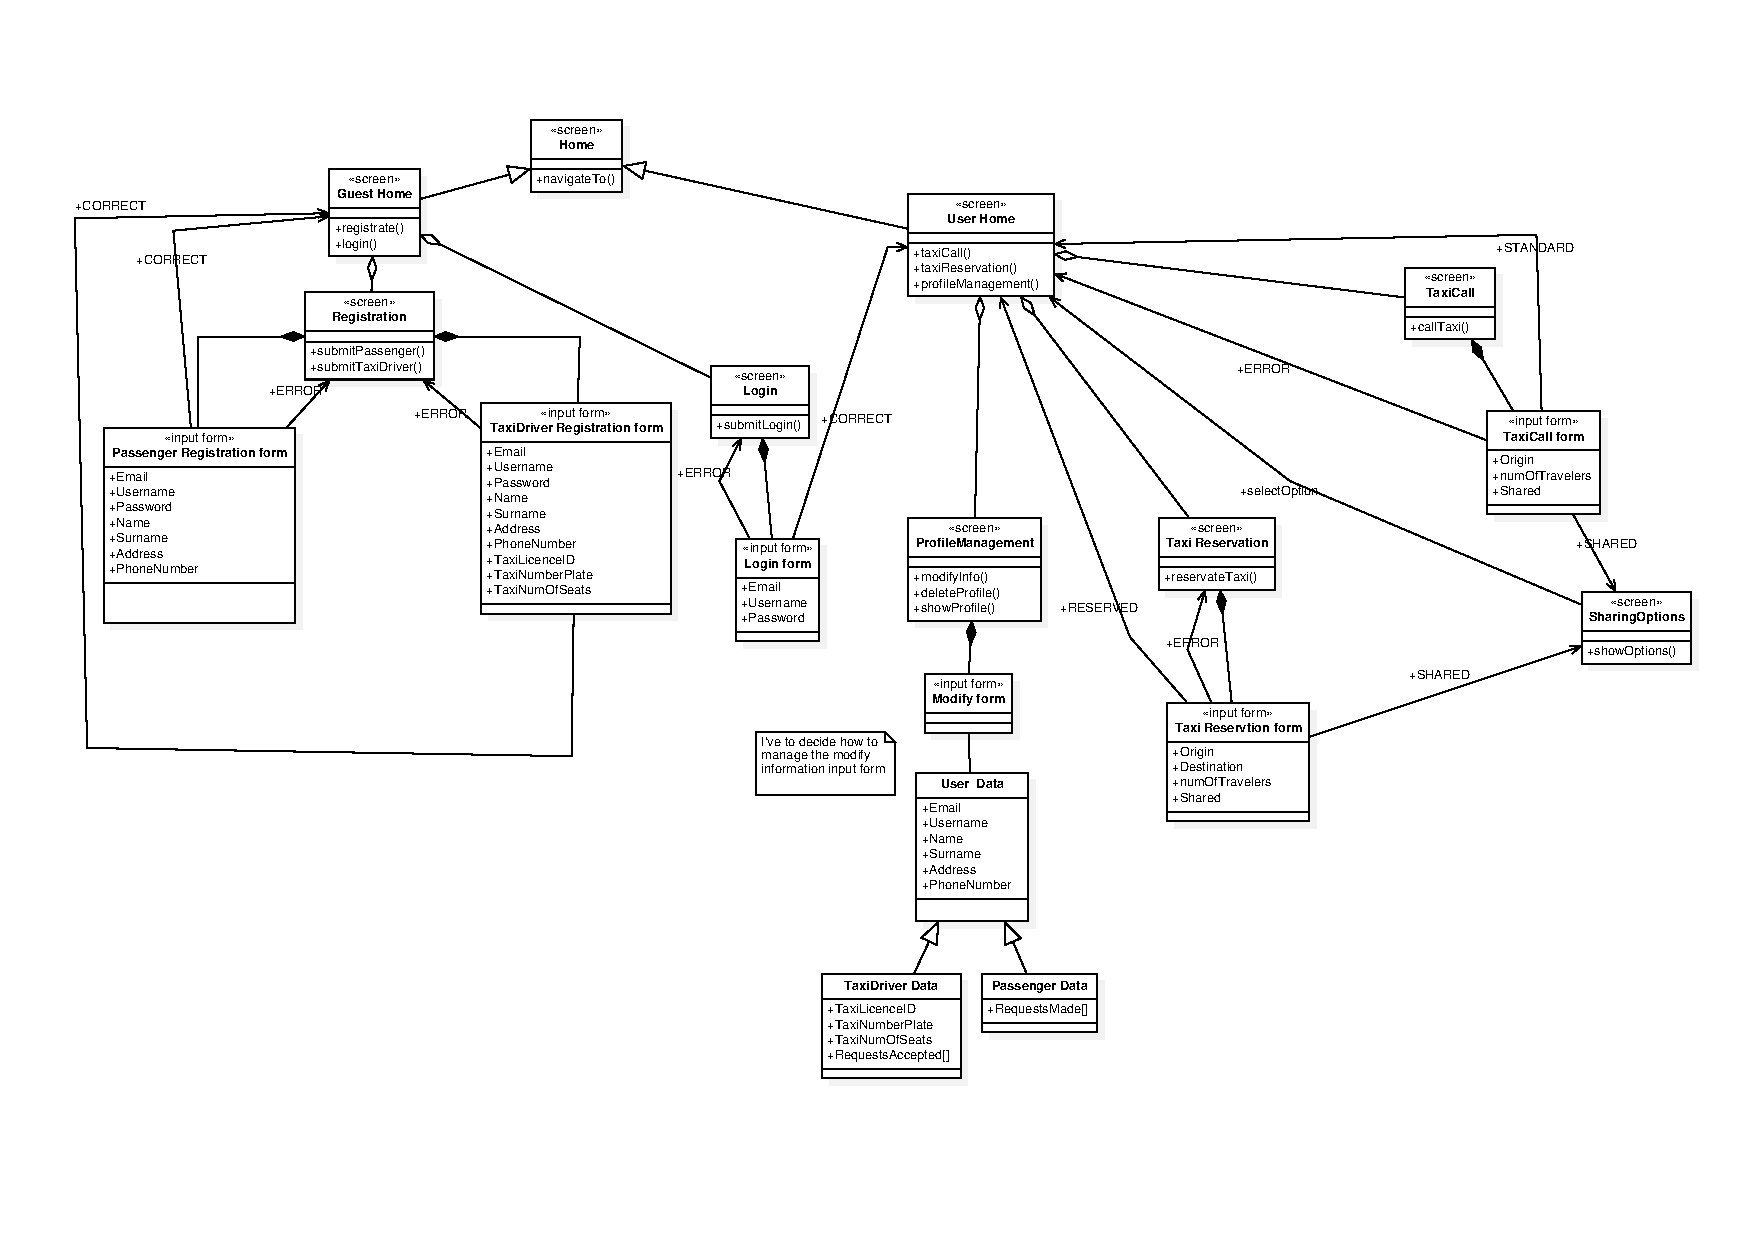
\includegraphics[width=\textwidth]{diagrams/UXdiagramSE2}
\caption{The UX diagram.}
\label{fig:ux-diagram}
\end{figure}

\FloatBarrier
\section{User Interface concept}

\subsection{Web interface}
These mock-ups show how the user interface for the web application should look like on web browser, also with the possibility to choose the language in every screen.

\begin{figure}[h]
\centering
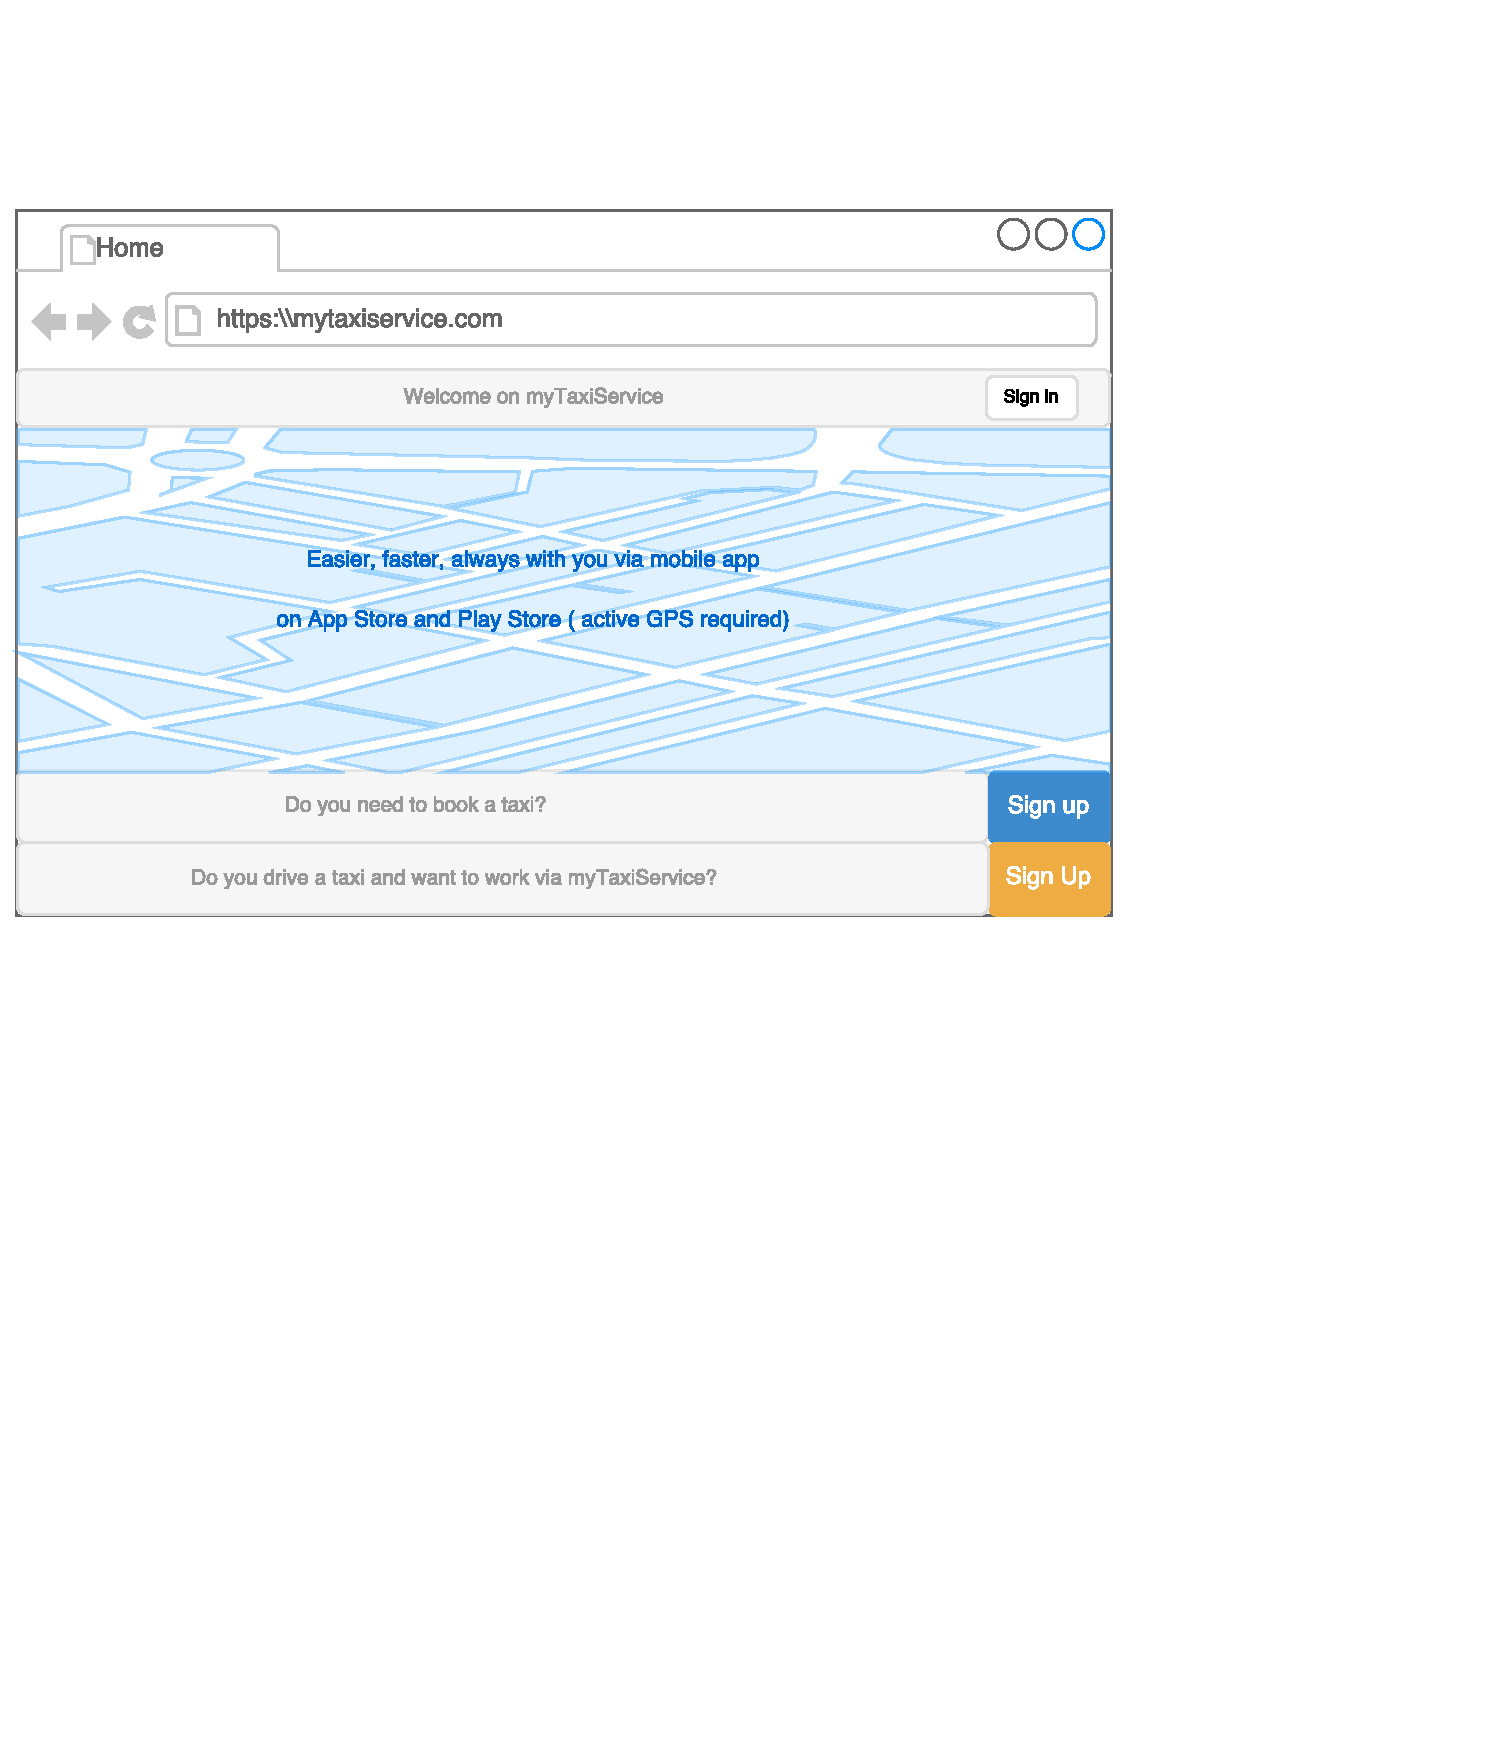
\includegraphics[width=0.7\textwidth]{mockup/web/GuestHome}
\caption{The home page of myTaxiService before log-in or registration.}
\label{fig:mockup-guesthome}
\end{figure}

\begin{figure}[h]
\centering
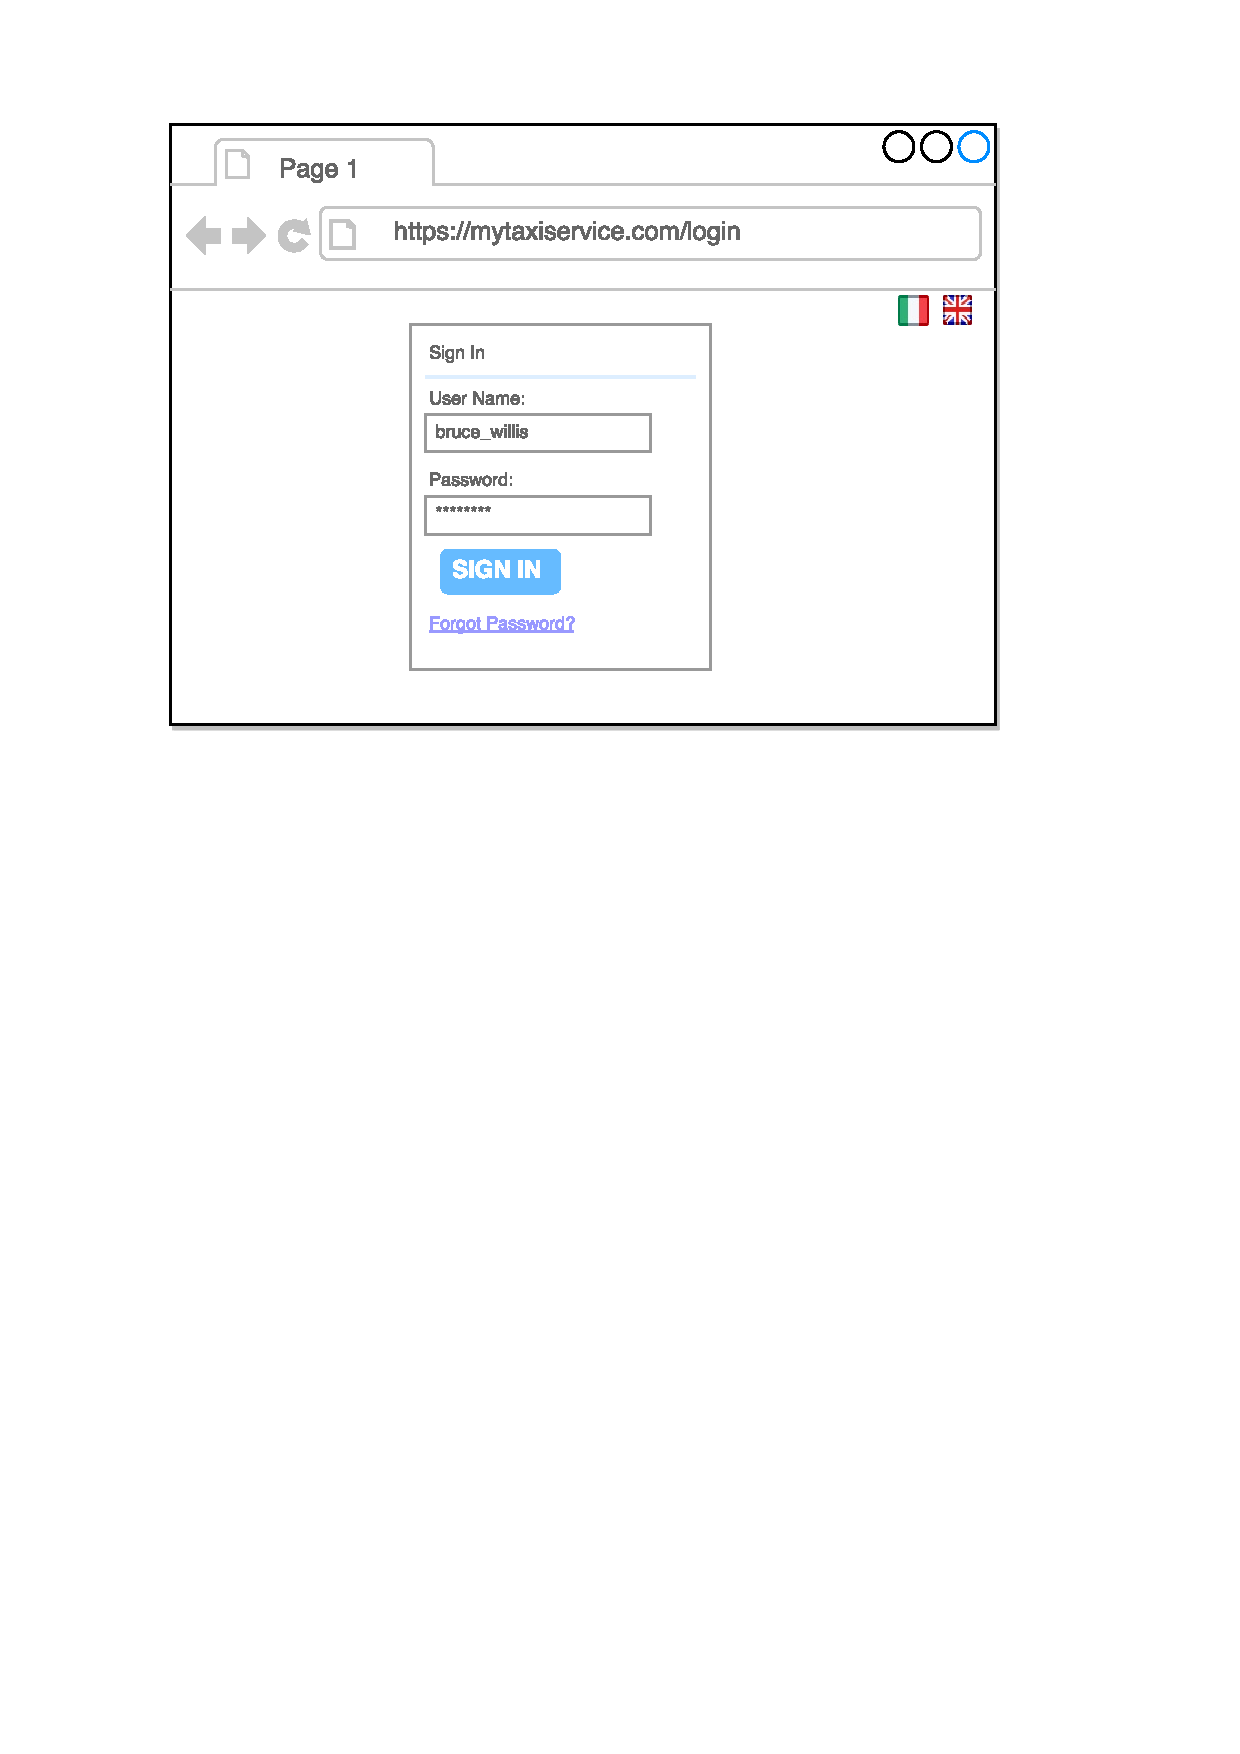
\includegraphics[width=0.7\textwidth]{mockup/web/Login_browser}
\caption{Login screen for the web application.}
\label{fig:mockup-login-browser}
\end{figure}

\begin{figure}[h]
\centering
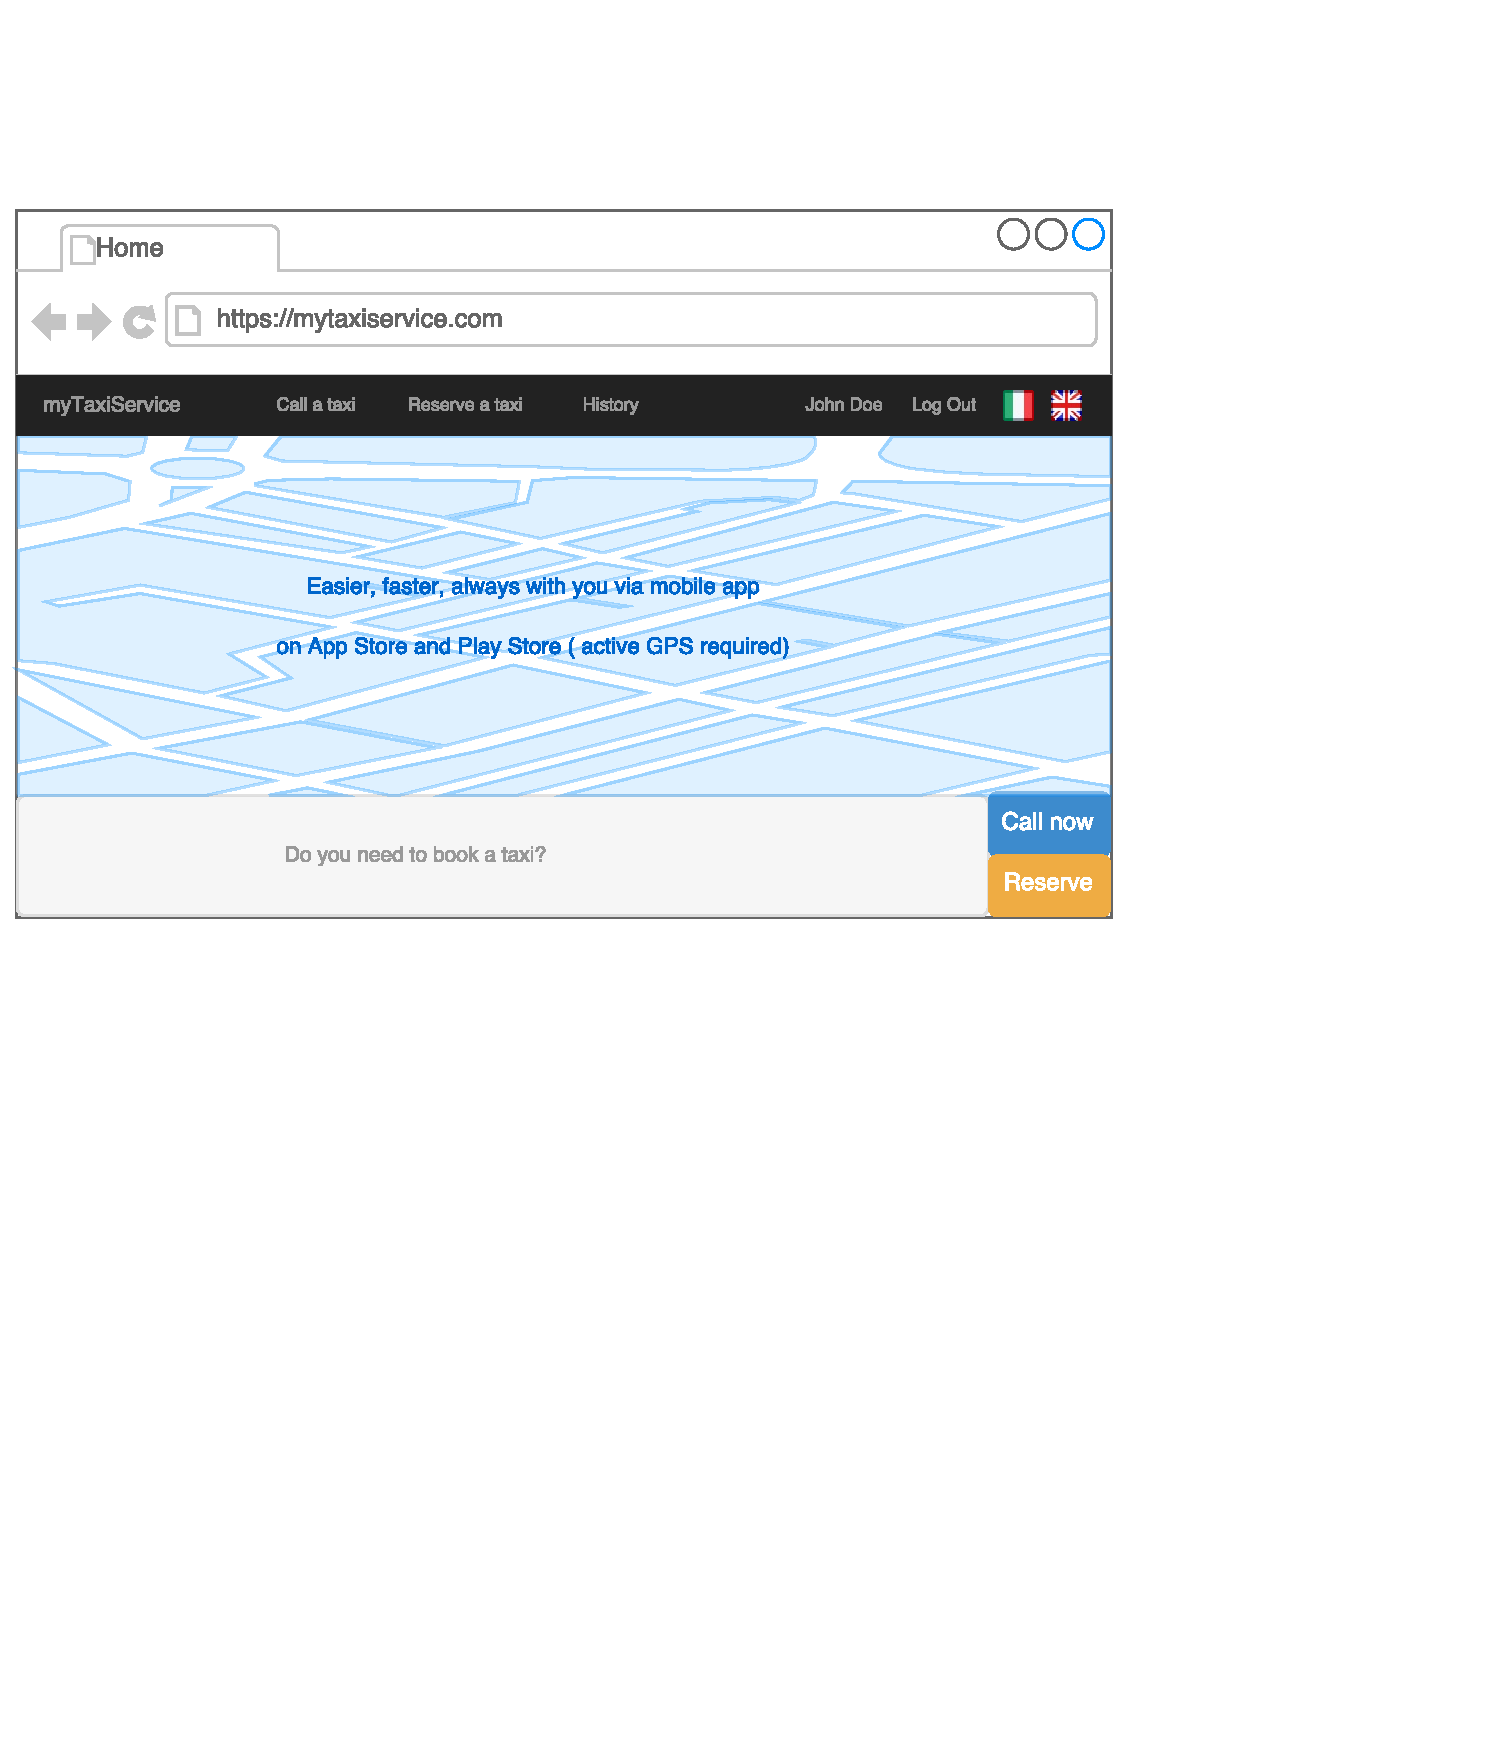
\includegraphics[width=0.8\textwidth]{mockup/web/UserHome}
\caption{Home page for the logged in passengers linking to all the functionalities.}
\label{fig:mockup-userhome}
\end{figure}

\begin{figure}[h]
\centering
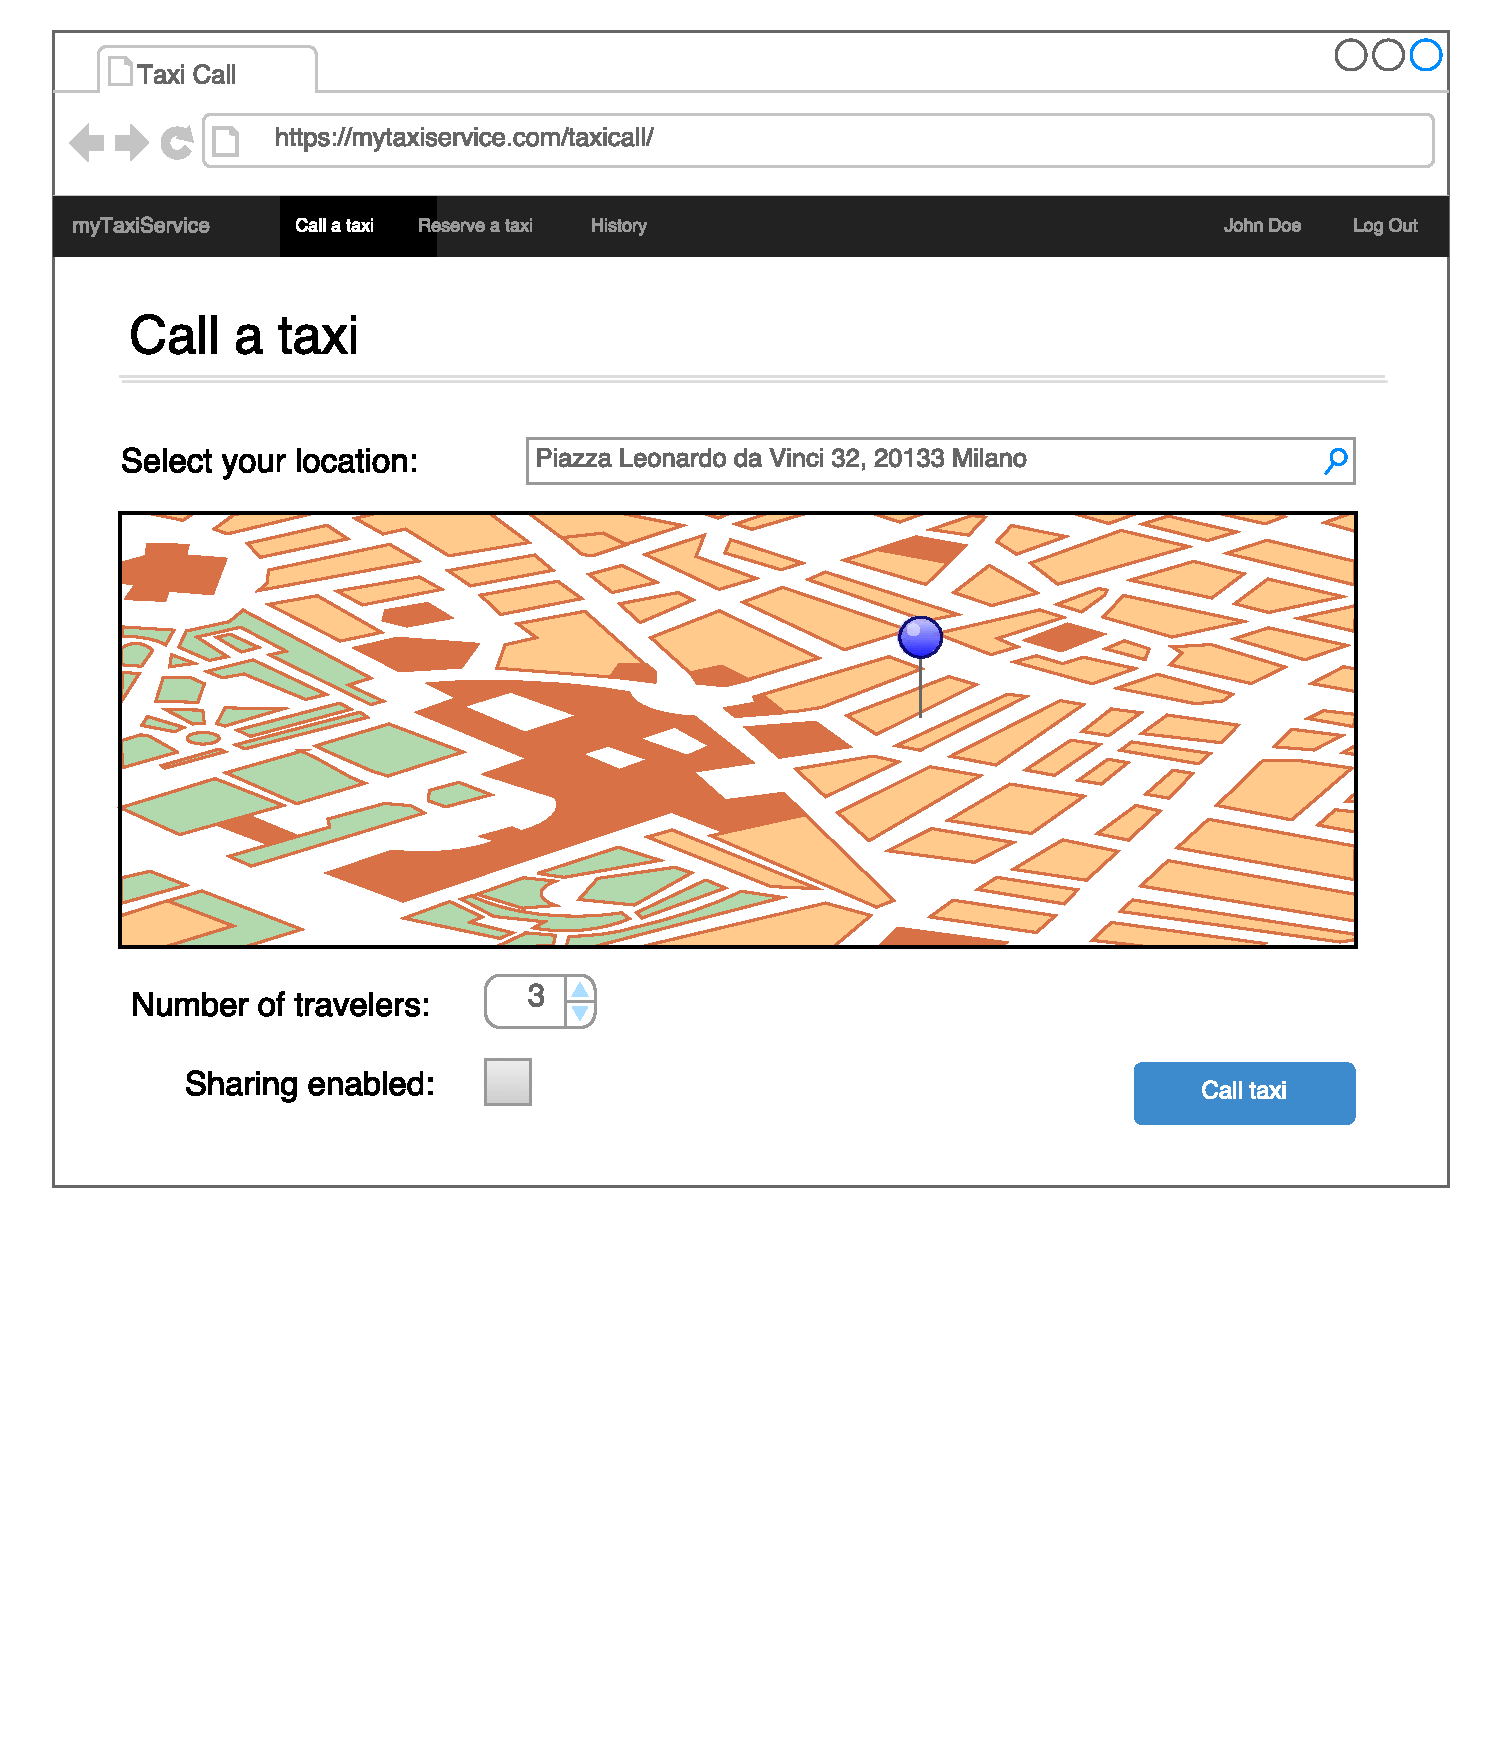
\includegraphics[width=0.8\textwidth]{mockup/web/TaxiCallBrowser}
\caption{Taxi call screen in the web application.}
\label{fig:mockup-taxicall-browser}
\end{figure}

\begin{figure}[h]
\centering
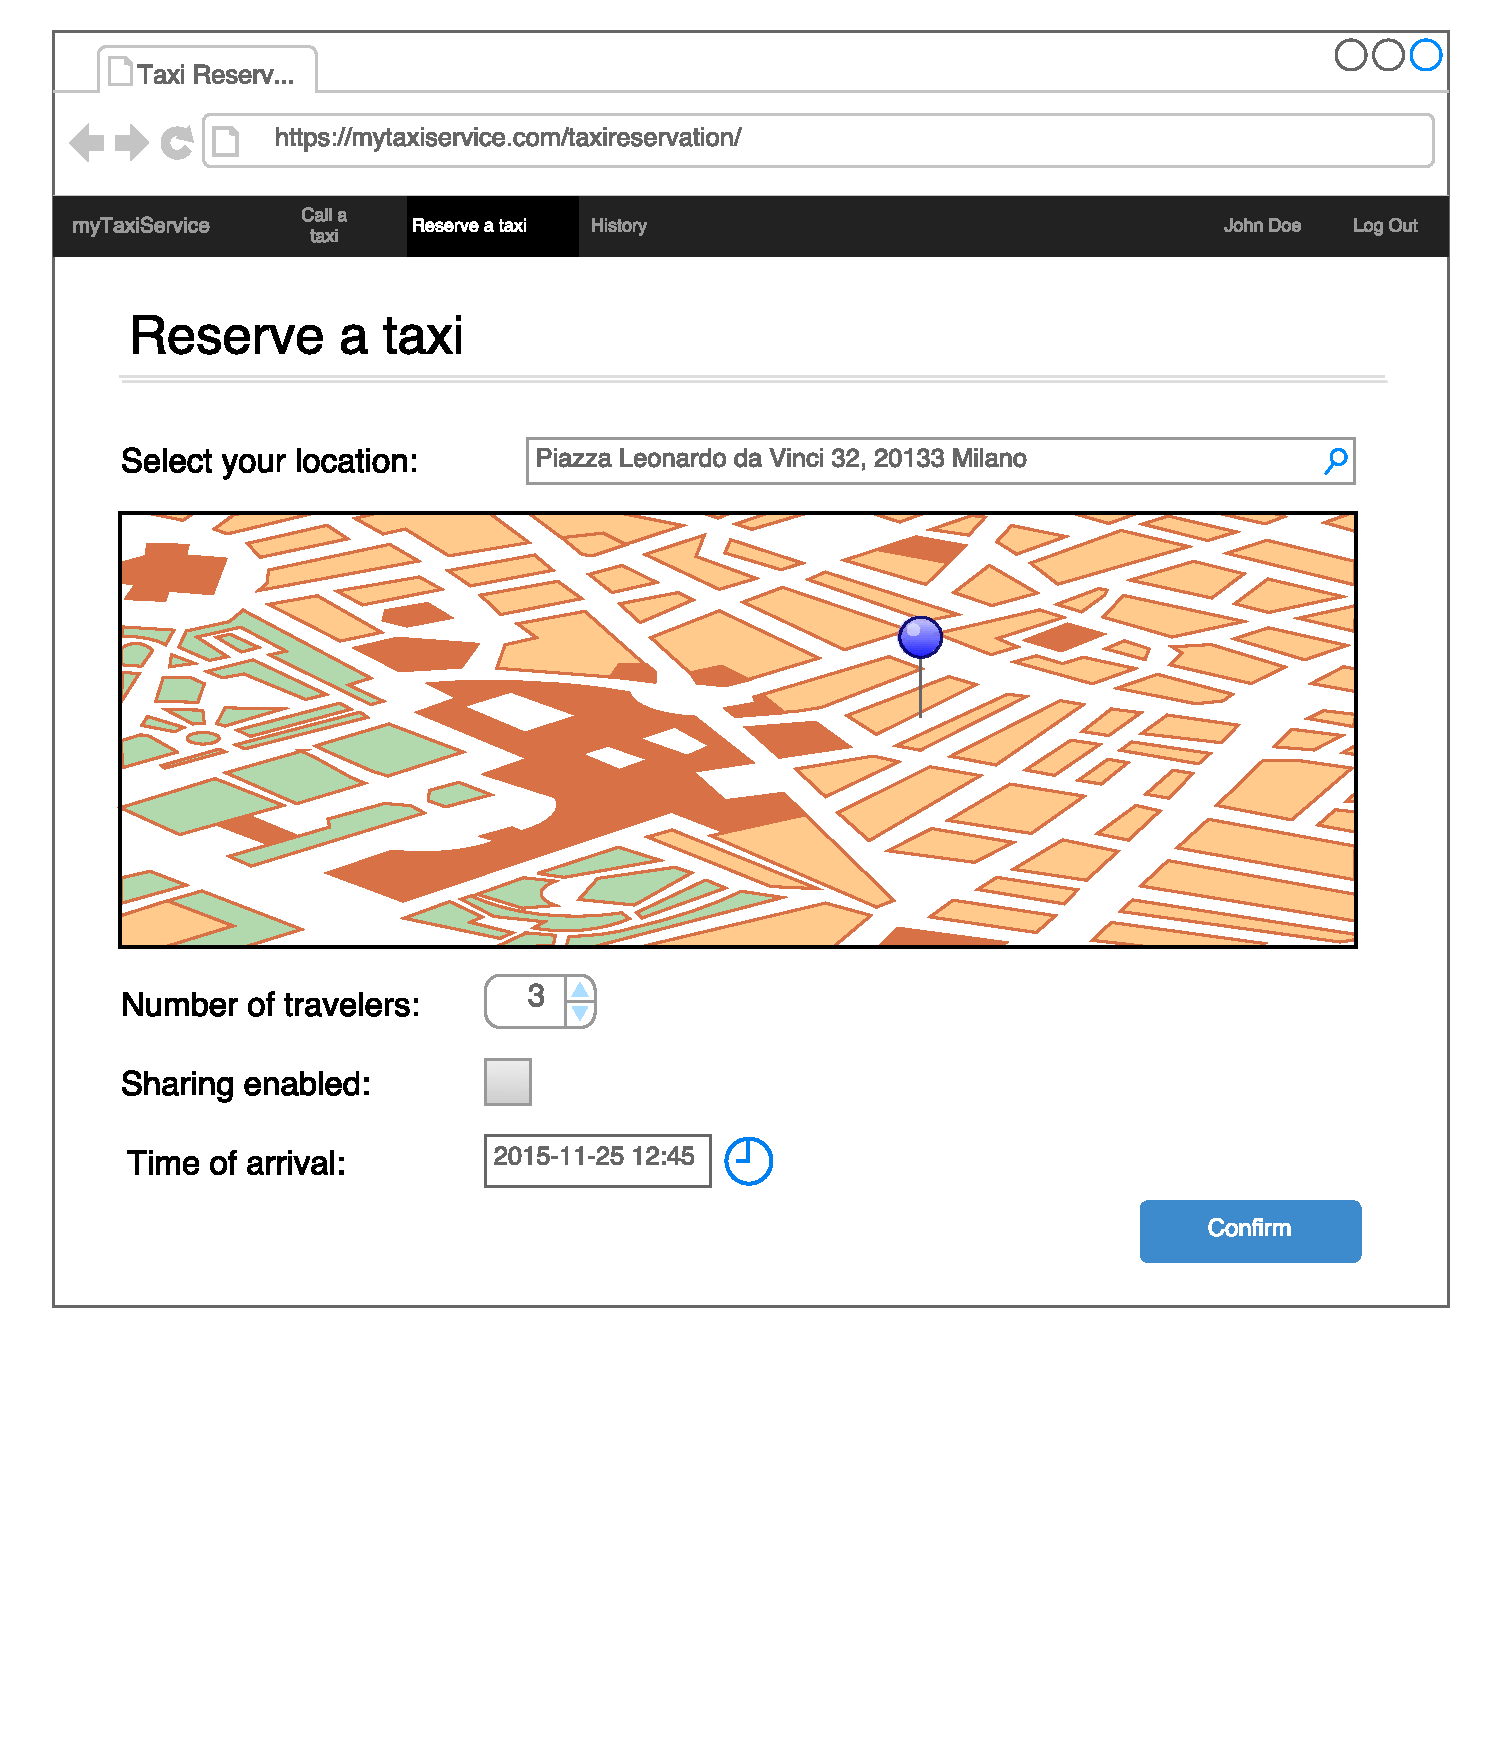
\includegraphics[width=0.8\textwidth]{mockup/web/TaxiReservationBrowser}
\caption{Taxi reservation screen in the web application.}
\label{fig:mockup-reservation-browser}
\end{figure}

\begin{figure}[h]
\centering
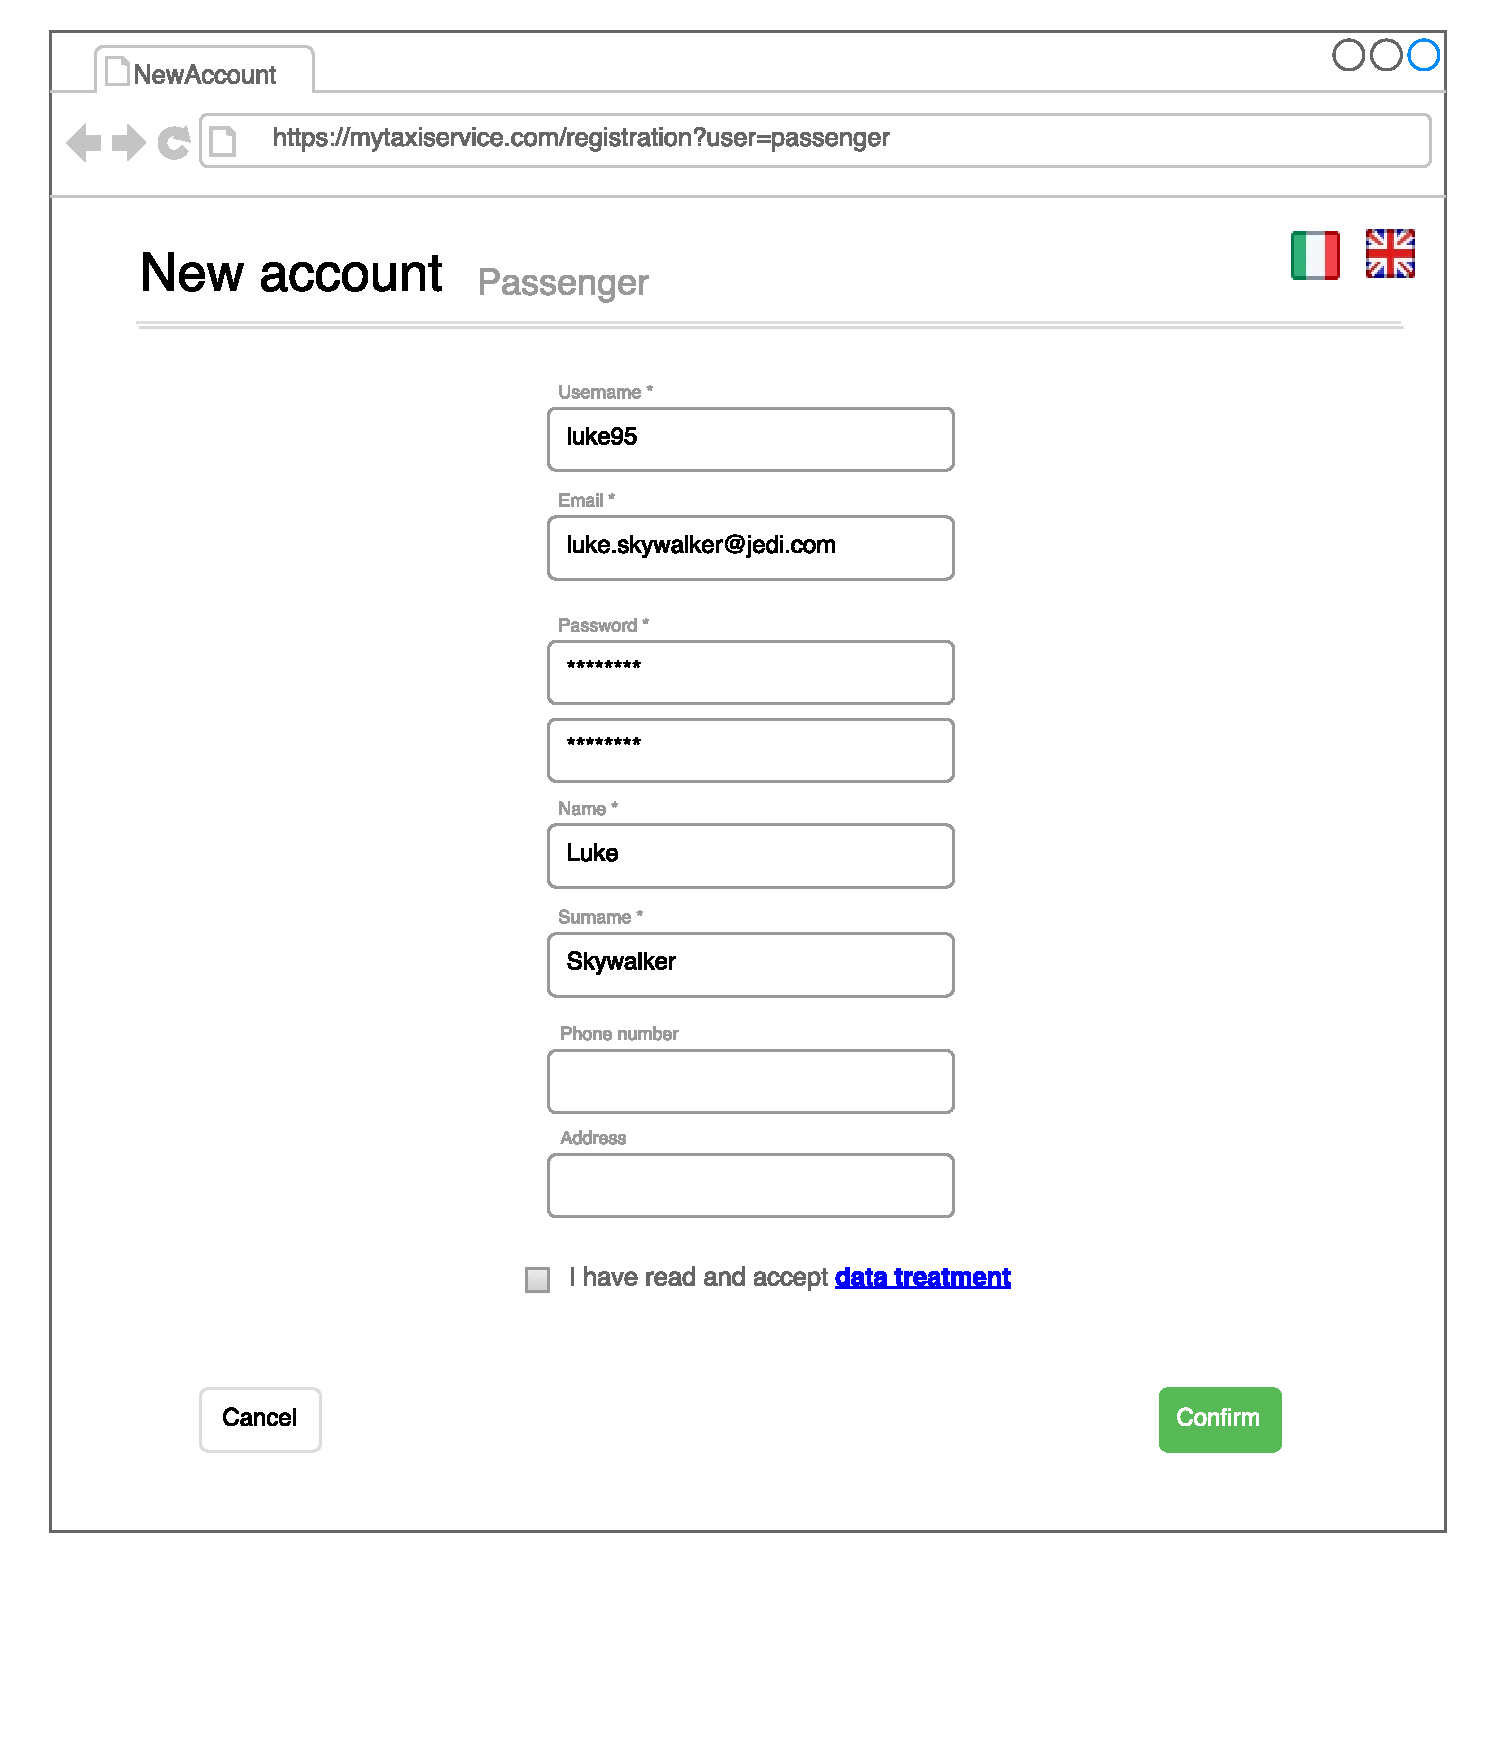
\includegraphics[width=0.9\textwidth]{mockup/web/Registration}
\caption{Registration screen for new users in the web application.}
\label{fig:mockup-registration}
\end{figure}

\FloatBarrier
\subsection{Mobile interface}
These mock-ups show how the interface of the myTaxiService mobile application will look like.

\begin{figure}[h]
    \centering
    \begin{subfigure}{0.45\textwidth}
        \centering
        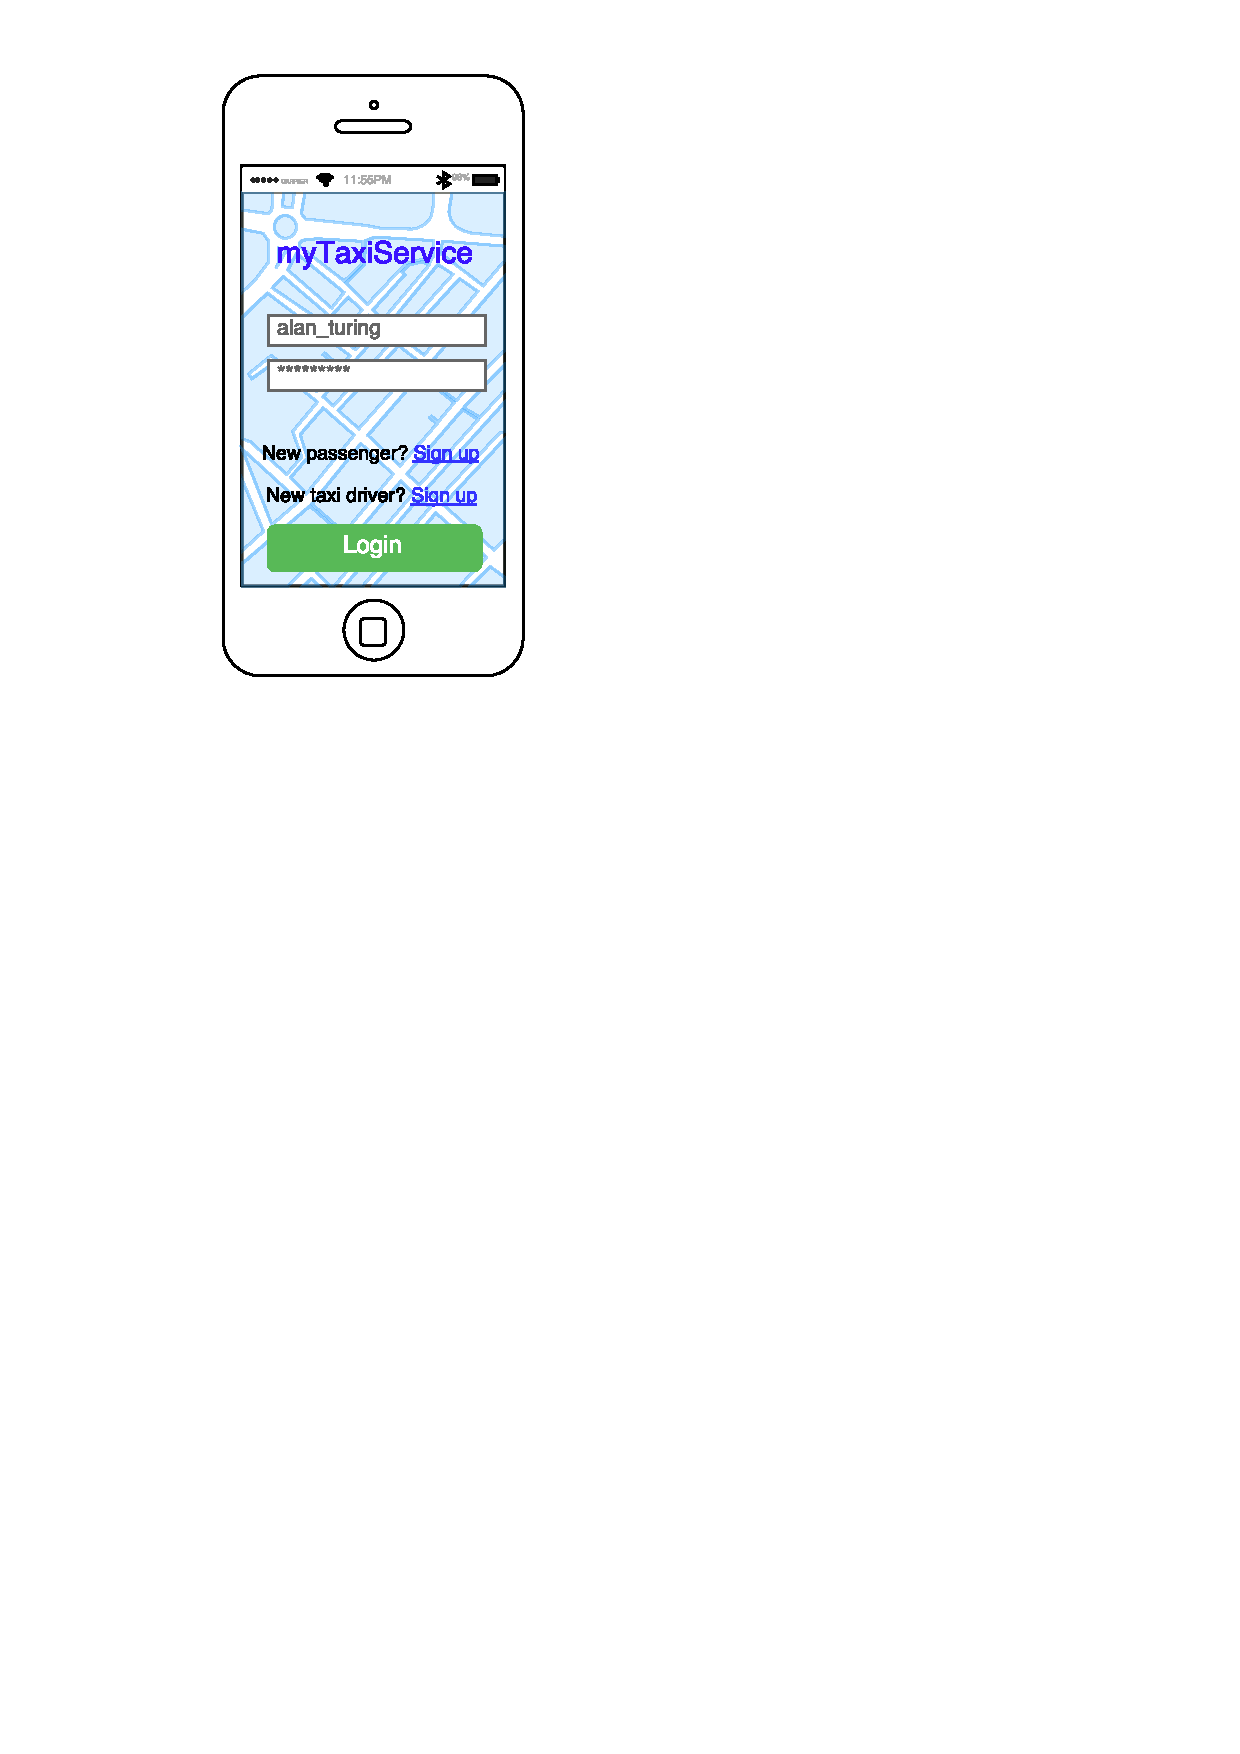
\includegraphics[width=\textwidth]{mockup/app/MobileLogin}
        \caption{Initial login screen on the mobile application. This screen also presents the option for signing up if the user does not have an account.}
        \label{fig:mockup-login-mobile}
    \end{subfigure}
    \hspace{1cm}
    \begin{subfigure}{0.45\textwidth}
        \centering
        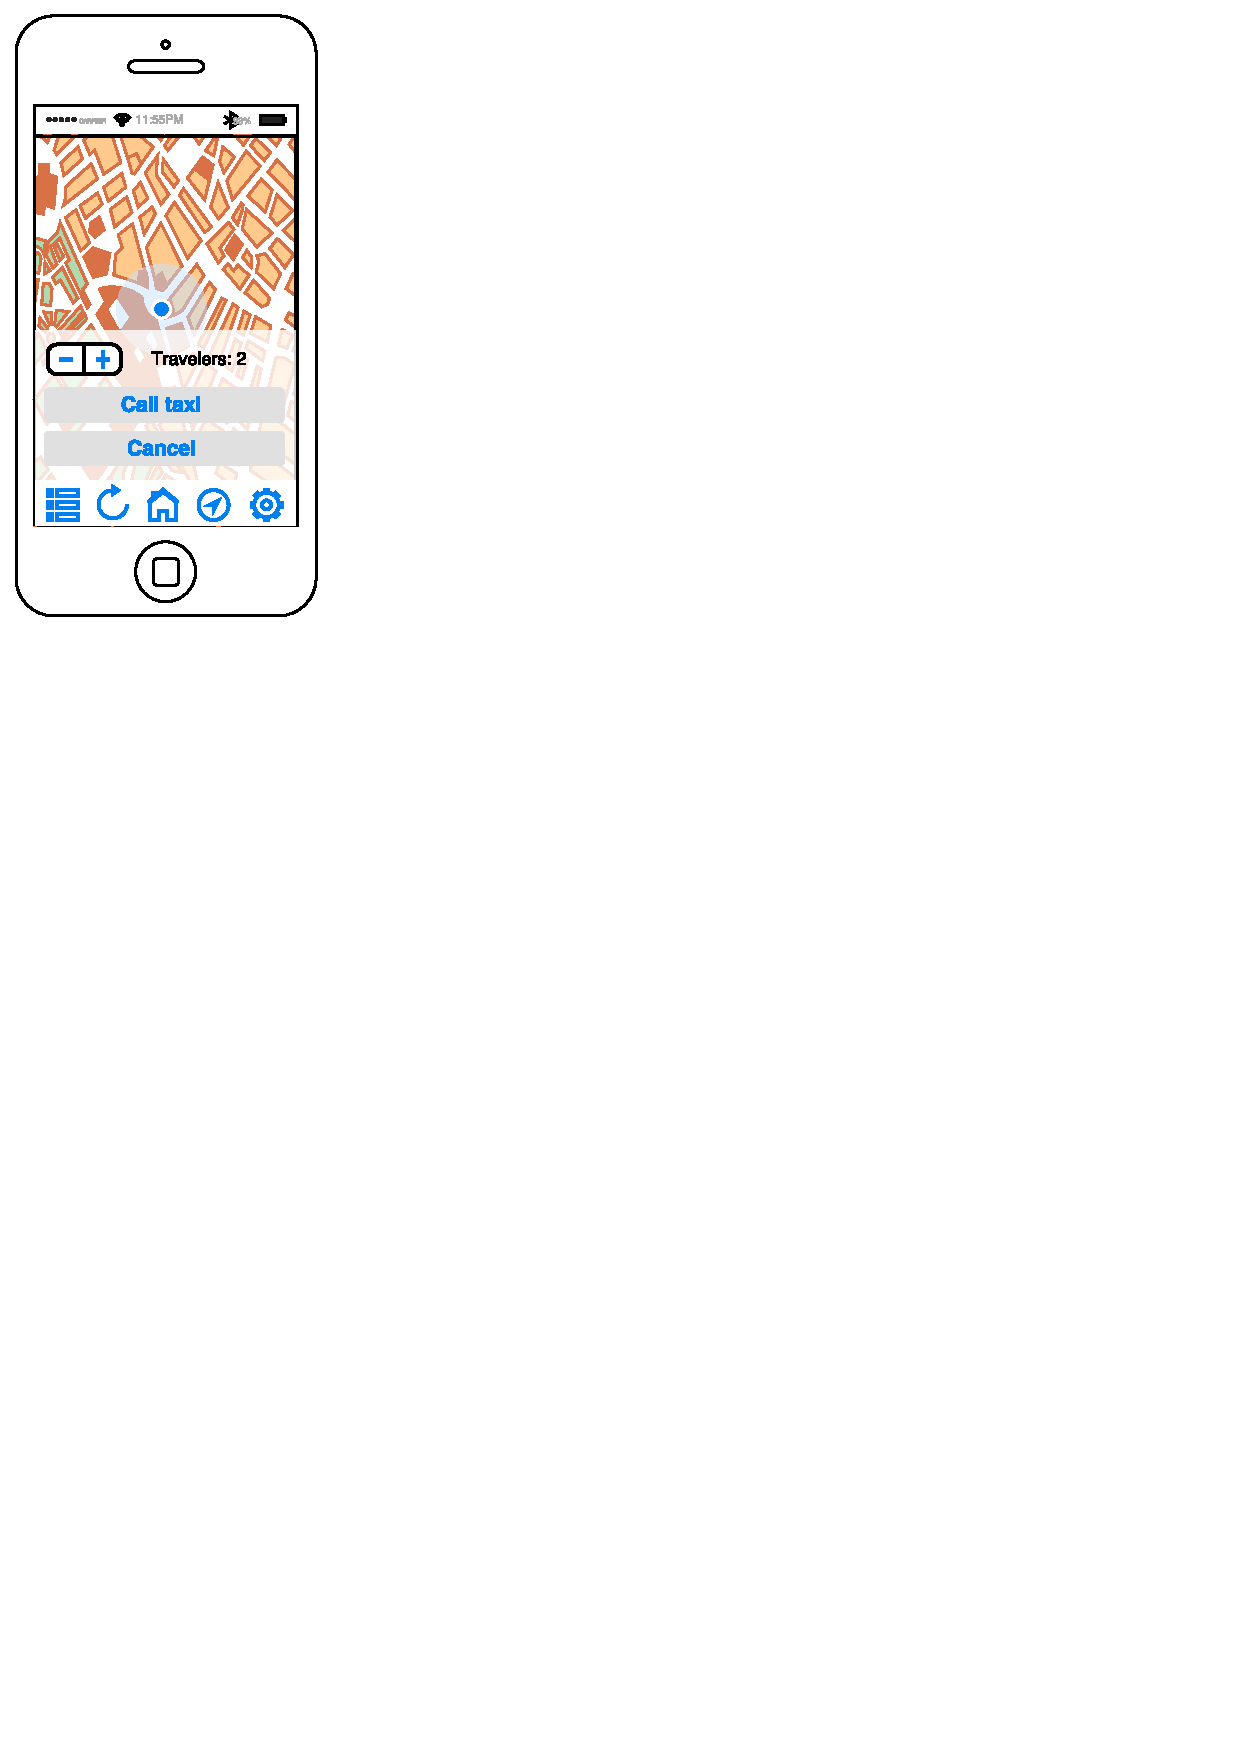
\includegraphics[width=\textwidth]{mockup/app/TaxiCall}
        \caption{Taxi call interface for the mobile application. The passenger may check if his location is correct and call a taxi specifying the number of travelers.}
        \label{fig:mockup-taxicall-mobile}
    \end{subfigure}
    \caption{Login and taxi call screens for the mobile application.}
\end{figure}

\begin{figure}[h]
    \centering
    \begin{subfigure}{0.45\textwidth}
        \centering
        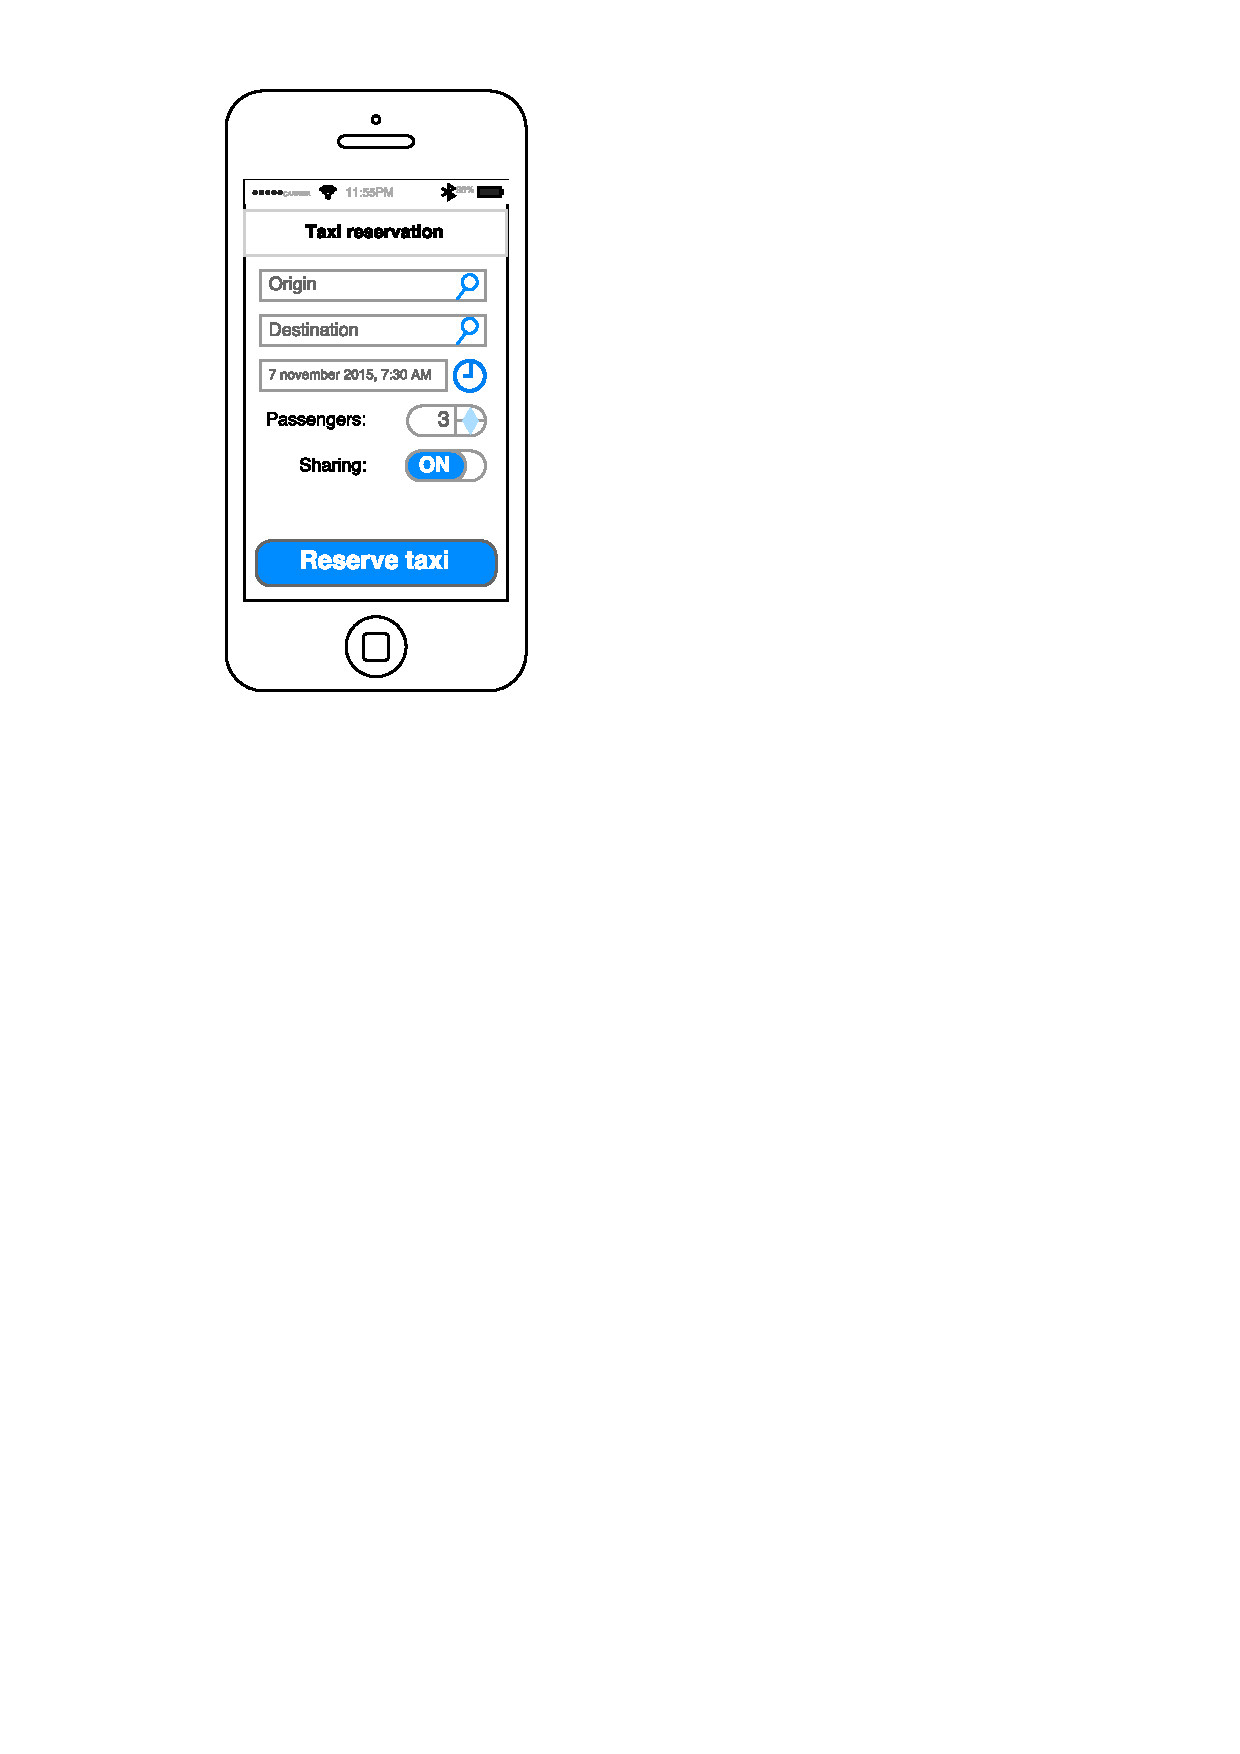
\includegraphics[width=\textwidth]{mockup/app/TaxiReservation}
        \caption{Taxi reservation screen for the mobile application.}
        \label{fig:mockup-reservation-mobile}
    \end{subfigure}
    \hspace{1cm}
    \begin{subfigure}{0.45\textwidth}
        \centering
        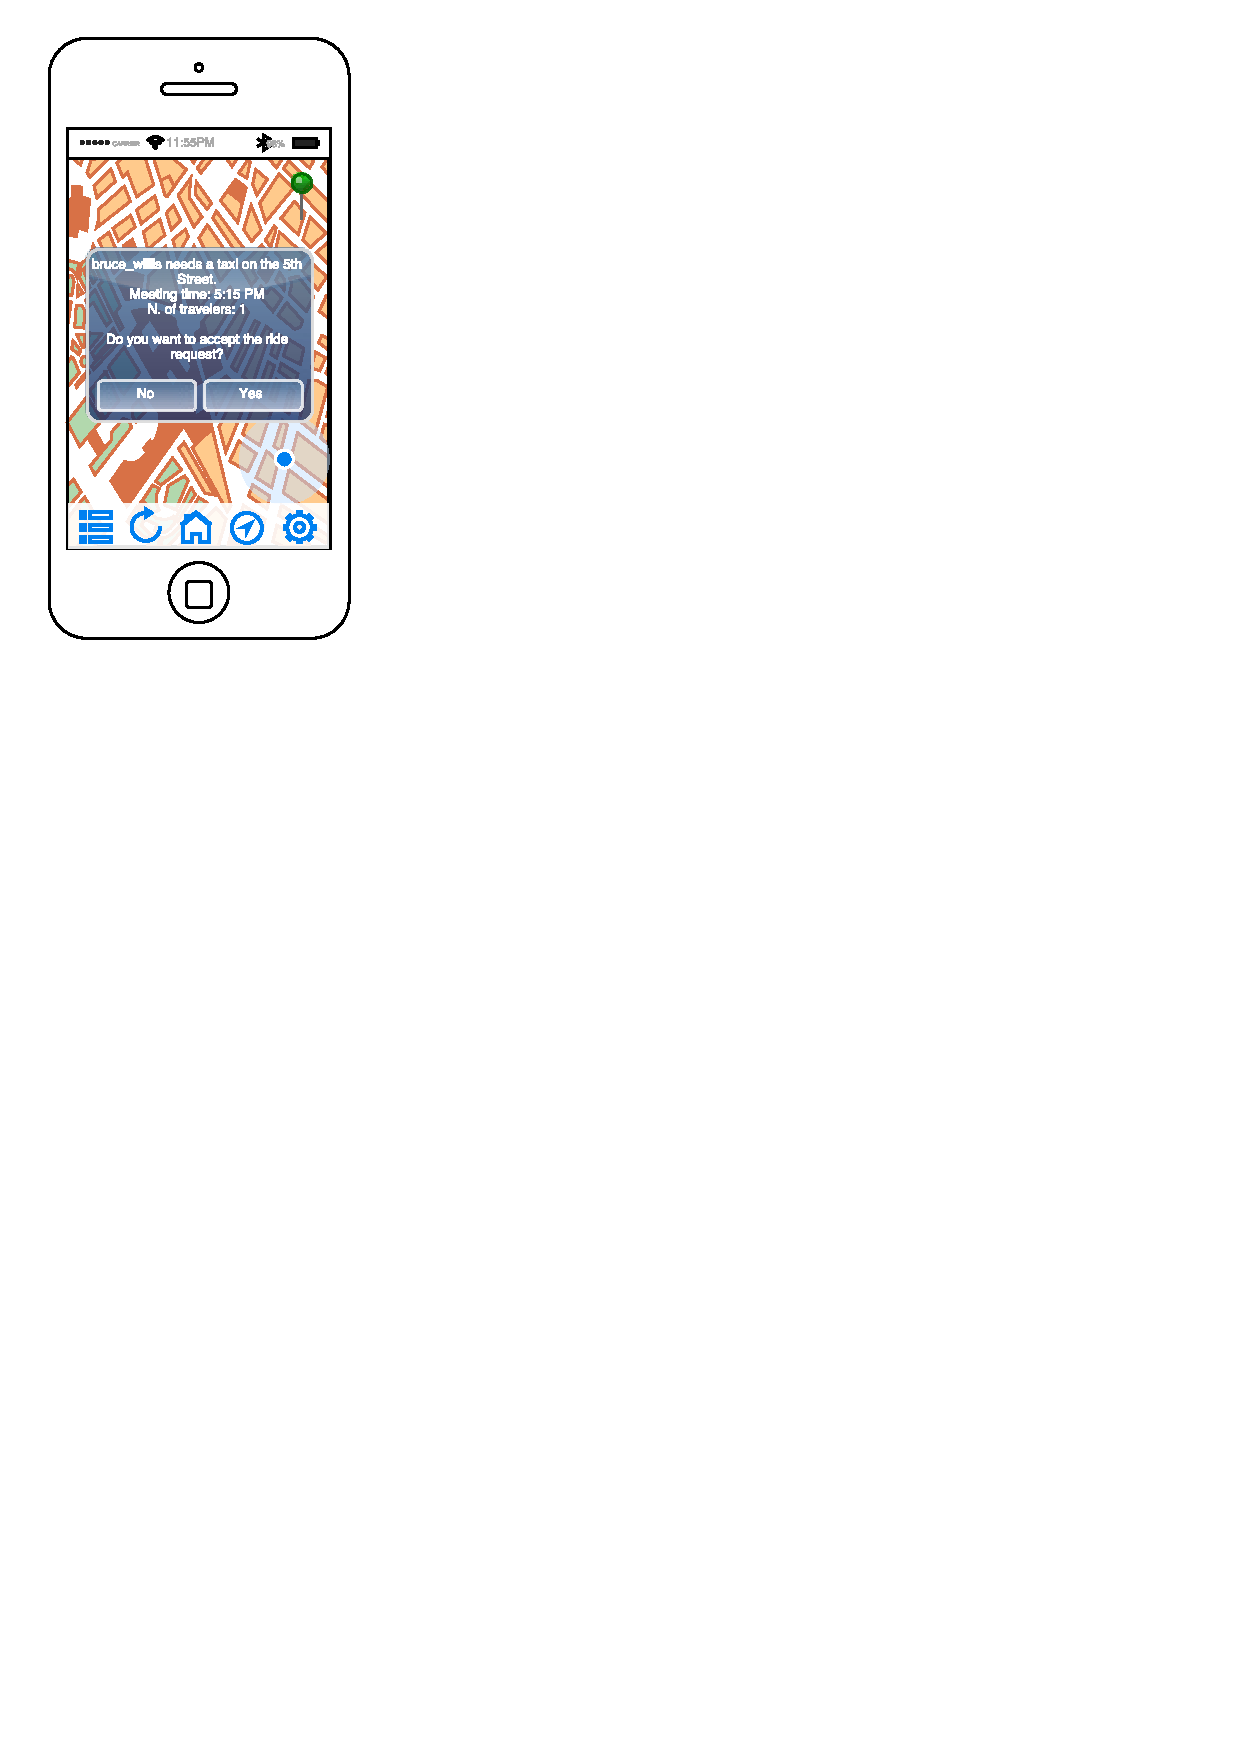
\includegraphics[width=\textwidth]{mockup/app/RideRequest}
        \caption{Ride request notification for taxi drivers in the mobile application.}
        \label{fig:mockup-riderequest-mobile}
    \end{subfigure}
    \caption{Taxi reservation and ride request screens for the mobile application.}
\end{figure}
